\chapter{Method}
\label{cha:method}
This chapter describes the proposed system for arrival time prediction
and event detection, and its implementation.

\section{System Description}
This section formally describes the system piece-wise. On a conceptual
level, the system assumes that similar trajectories, with respect to their motion patterns, should arrive at
approximately the same time. When presented with a new trajectory, the system
finds previously observed trajectories with similar motion patterns,
and predict arrival times based on the most similar one. 

The current system description assume that each trajectory represents
a motion pattern (motion pattern clusters has a single trajectory).

\section{Trajectory Model}
To find similar trajectories, a trajectory similarity metric 
is needed. The similarity metric need to be well defined for
trajectories of different temporal lengths, and unevenly
distributed observations.

\subsection{Synchronisation Model}
One notion of similarity between trajectories is some aggregation of
local similarities. Consider the local distance from an observation on trajectory
$\traj_{i}$ to trajectory $\traj_{j}$ as the distance of the orthogonal
projection onto $\traj_{j}$, as illustrated in Figure~\ref{fig:trajectory-projection}.
\begin{figure}
  \centering
  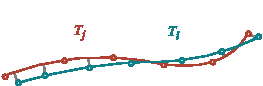
\includegraphics[scale=2.5]{trajectory-projection}
  \caption{An illustration of local distances from $\traj_2$ to
  $\traj_1$ as point-wise orthogonal projections.}\label{fig:trajectory-projection}
\end{figure}
This approach would eliminate the need to align observations before
comparison. However, it requires a continuous trajectory
representation, while trajectories are observed as discrete samples.
A step toward this is seeing observations as samples from a continuous function
$\traj_{k} = \tilde{f}_{k}(t)$, which describes the trajectory as a function of
time. While continuous, this description is based on specific time
points, but the \textit{exact points in time} of observations are not
relevant, since trajectories for a single segment are generated at many different
occasions. Instead, consider observations as samples from the function
as $\traj_{k} = \modelf_{k}(\synchspace)$, where $\synchspace = [0, 1]$ is the \textit{progress} from
start ($\synchspace = 0.0$) to finish ($\synchspace = 1.0$) of
a trajectory. This function makes it possible to talk about observations based on
progression for any trajectory, regardless of the exact observation time points. 

Assuming the samples are jointly Normally distributed, and
that $\modelf$ is smooth, a GP can be fit to the
observations to approximate $\traj_{k} = \modelf_{k}(\synchspace)$, with
independent outputs. Finding a projection for an observation $\newobs$ onto trajectory
$\traj_{k}$ can now be seen as finding how far along the trajectory $\newobs$
would have traveled. More precisely, finding the $\synchspace$ that $\newobs$
corresponds to. Under the assumption that $\synchspace \sim
\mathcal{N}(\mu_{\synchspace}, \Sigma_{\synchspace})$, a multivariate
GP is used to model $\synchspace = \synchf_{k}(\obs)$, which maps $\newobs$ onto the
progress relative to $\traj_{k}$. When considering progress along a
segment, the current velocity does not matter. Hence, the domain of
$\synchf_{k}$ is the subspace $\posspace = (p_x, p_y)$ of $\statespace$, and
consequently $\statespace$ is collapsed into $\posspace$ before
mapping onto $\synchspace$. The projection onto $\traj_{k}$ is
finally given by the composition $\synchedobs = (\modelf \circ
\synchf)(\obs)$, illustrated in Figure~\ref{fig:synch-model}.
\begin{figure}
  \centering
  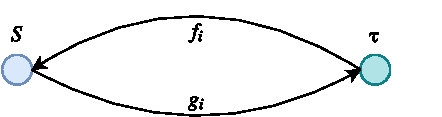
\includegraphics[scale=1.5]{synch-model}
  \caption{An illustration of the mappings involved when synchronising
    trajectories. Trajectories are observed in the \textit{state space} $\statespace =
(p_x, p_y, v_x, v_y)$, containing position and velocity. Then projected by $p$ onto the
    subspace $\posspace = (p_x, p_y)$. Then onto
    $\synchspace$ by $\synchf_{k}$, and finally back onto $\statespace$ by
    $\modelf_{k}$.}\label{fig:synch-model}
\end{figure}
In light of the these results, let $\model_{synch}^{(k)} = (\modelf_{k},
\synchf_{k})$ be the \textit{synchronisation model} of $\traj_{k}$.

The final step is to formulate a local similarity metric from the
projections and aggregate this into a global one.
While it is intuitive to define the local similarity as the Euclidian distance $||E[\synchedobs]
- \newobs||_{2}$, this approach does not consider the  uncertainty in $\synchedobs$. 
Consider instead the data log likelihood
\begin{equation}
  \label{eq:model-log-likelihood}
  \begin{split}
    \log P(\synchspace \vert \newobs, \model_{synch}^{(k)})
    & = -\frac{1}{2}(\synchspace - \mu(\newobs)){[\Sigma(\newobs)]}^{-1}(\synchspace - \mu(\newobs)) \\
    & = -\frac{1}{2}\log{|\Sigma(\newobs)|}+C,
  \end{split}
\end{equation}
where $\mu(\newobs)$ and $\Sigma(\newobs)$ are given by
equations~\ref{eq:gp-mean-function},
and~\ref{eq:gp-covariance-function} for a GP modeling $f_{k}$. The
likelihood measures how well $\model_{synch}^{(k)}$ explains observation
$\newobs$, and is a measure of similarity. Assuming that all models
are equally probable a priori, Bayes theorem gives
\begin{equation}
  \label{eq:model-posterior}
    P(\model_{synch}^{(k)} \vert \newobs, \synchspace)
     \propto P(\synchspace \vert \newobs, \model_{synch}^{(k)})  
    P(\model_{synch}^{(k)}) 
    \propto P(\synchspace \vert \newobs, \model_{synch}^{(k)})
\end{equation}
and the most similar model can consequently be chosen by $M_{c} = \underset{k}{\mathrm{argmax}} \log
P(\model_{synch}^{(k)} \vert \newobs, \synchspace)$. 
This similarity metric properly considers the uncertainty in
$\synchedobs$, and generalises to a global one
for an entire trajectory by letting $\newobs$ be
\[\newobs =
  \begin{pmatrix}
    p_{x}^{1} & p_{y}^{1} & v_{x}^{1} & v_{y}^{1} \\
    p_{x}^{2} & p_{y}^{2} & v_{x}^{2} & v_{y}^{2} \\
    \vdots  & \vdots  & \vdots & \vdots  \\
    p_{x}^{m} & p_{y}^{m} & v_{x}^{m} & v_{y}^{m} \\
  \end{pmatrix}.
\]

\begin{equation}
  P(\model_{k} \vert \synchedobs = \newobs)
   \propto P(\synchedobs = \newobs \vert \model_{k}, \obs) P(\model_{k}
  \vert \obs) = P(\synchedobs = \newobs \vert \model_{k})
\end{equation}

%Having a distribution over models will also prove useful when making arrival time predictions. 
\subsection{Learning the Synchronisation Model}
Learning a synchronisation model $\model_{synch}^{(k)}$ means learning
$\modelf_{k}$ and $\synchf_{k}$ by MAP estimation. However, there are
more constraints on the functions than can be formulated in
priors. In particular, a critical property of $\synchf_{k}$
is that it should be monotonically increasing in the direction of progression,
and stationary orthogonal to it. This is intuitively explained by the fact that a
vehicle is no closer to its destination should it drive more to the
left or right on a road; only the progression \textit{along} the road
matters. Formally, this is required for the projection onto a
trajectory to be orthogonal. To enforce this property, data augmentation is used.

When training GPs using a stationary kernel function, it is assumed
that the data is uniformly distributed, which is not the case for the
data set used. Recall the function $\synchf_{k} : \posspace \mapsto
\synchspace$. In this case, the data is assumed to be uniformly
distributed in $\posspace$, but as described in Chapter~\ref{ch:data},
all data is collected approximately uniform in \textit{time}. This causes many
observations to be generated in close proximity during stand-stills, which skews the
learning of the kernel lengthscale parameters to small values. To
make data approximately uniformly distributed spatially instead and 
avoid this problem, a technique called \textit{stop compression} is used.

\subsubsection{Data Augmentation}
\label{sec:data-augmentation}
For reasons previously described, $\synchf_{i}$ should be monotonically increasing in
the direction of progression and stationary orthogonal to it.
To enforce learning such a function, each
observation $\obs_{i}^{(i)}$ for a trajectory $\traj_{i}$is duplicated by placing a normal distribution
over it, orthogonal to the spatial progression vector ${(\obs^{(i+1)}_x -
  \obs^{(i)}_x, \obs^{(i+1)}_y - \obs^{(i)}_y)}^T$, and drawing several samples
with the same progression as $\obs^{(i)}$. This process is illustrated in
Figure~\ref{fig:traj-without-support-data} and
Figure~\ref{fig:traj-with-support-data}.
\begin{figure}
  \begin{minipage}{.46\textwidth}
    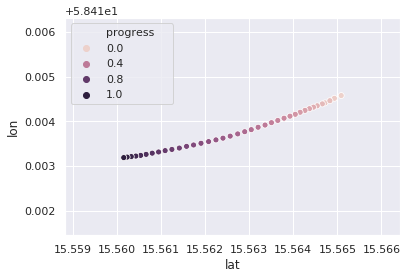
\includegraphics[scale=0.48,width=\textwidth]{traj-without-support-data2}
    \caption{Spatial progression of a trajectory
      before data augmentation.}\label{fig:traj-without-support-data}
  \end{minipage}
  \hspace{5pt}
  \begin{minipage}{.46\textwidth}
    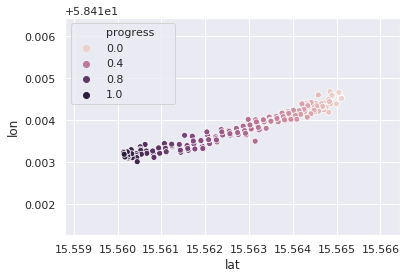
\includegraphics[scale=0.5,width=\textwidth]{traj-with-support-data2}
    \caption{Spatial progression of a trajectory
      after data augmentation. }\label{fig:traj-with-support-data}
  \end{minipage}
\end{figure}

\subsubsection{Stop Compression}
\label{sec:stop-compression}
Stop compression aggregates observations in close proximity into a
single observation through averaging. Observations within a radius of
$4$m are clustered into a single observation with the mean value of
the clustered observations. An example of this is seen
Figure~\ref{fig:stop-compression-before} and Figure~\ref{fig:stop-compression-after}.
\begin{figure}
  \begin{minipage}{.46\textwidth}
    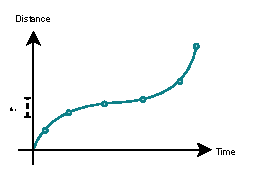
\includegraphics[scale=0.48,width=\textwidth]{stop-compression-before}
    \caption{Trajectory before stop compression. Several observations
      are very close spatially, but the data is
      approximately uniformly distributed temporally. }\label{fig:stop-compression-before}
  \end{minipage}
  \hspace{5pt}
  \begin{minipage}{.46\textwidth}
    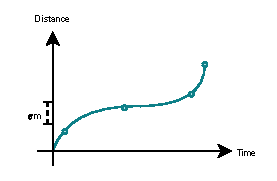
\includegraphics[scale=0.5,width=\textwidth]{stop-compression-after}
    \caption{Spatial progression of a trajectory
      after stop compression. The data is
      approximately uniformly distributed spatially.}\label{fig:stop-compression-after}
  \end{minipage}
\end{figure}

\subsection{Prediction Model}
Predicting arrival times can be seen as learning the remaining time of
a segment given a certain position. However, modeling it as $\arrtime
= \tilde{\predf_{k}}(p_x, p_y)$ would assume that every trajectory passes the
exact same positions. A better model is $\arrtime
= \predf_{k}(\synchspace)$, which instead depends on progression. Since the
progression represents similar trajectories and not a single one, this
model generalises much better. Assuming that $\arrtime \sim
\mathcal{N}(\mu_{\arrtime}, \Sigma_{\arrtime})$, a GP can model $\predf_{k}$, 
extending the synchronisation model to the \textit{trajectory model}
$\model_{k} = (\modelf_{k}, \synchf_{k}, \predf_{k})$, illustrated in Figure~\ref{fig:trajectory-model}.
\begin{figure}
  \centering
  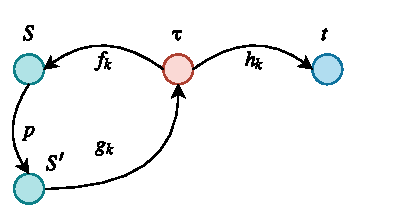
\includegraphics[scale=1.5]{trajectory-model}
  \caption{An illustration of the trajectory model, which models
    current state $\statespace$ and time left $\arrtime$ as functions of
    progress $\synchspace$. $P$ denotes orthogonal projection.}\label{fig:trajectory-model}
\end{figure}

\section{Arrival Time Predictions}
The arrival time predictions are modeled as a Mixture of Gaussian
Processes (MoGP), where each motion pattern model $\model_{k}$ induce a component. The
model predicts remaining time until arrival, and the probability of
the time remaining being $\arrtime$ for an observation $\obs$ is given by
the mixture
\begin{equation}
  P(\arrtime \vert \obs) = \sum_{k}P(\arrtime \vert \model_{k}, \obs)
  P(\model_{k} \vert \obs),
\end{equation}
where the component weights $P(\model_{k})$ are the same as
$P(\model^{(k)}_{synch})$, given by equation~\ref{eq:model-posterior}, 
since they are trained on the same
$\traj_{k}$. Since all components are Gaussian, 
$P(\arrtime \vert \obs)$ will have one mode for each component. The
point-estimate prediction of the model is taken to be the largest
mode, corresponding to the mean prediction of the most probable model.

% \begin{figure}[H]
%   \begin{minipage}{.46\textwidth}
%     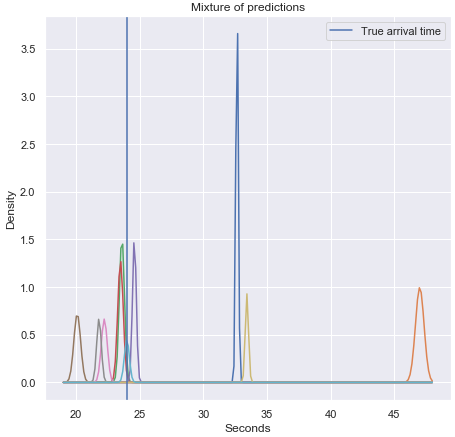
\includegraphics[width=\textwidth]{figures/mixture-start-of-traj.png}
%     \caption{Density of arrival time predictions at 
%       the start of a segment.}\label{fig:mixture-start-of-traj}
%   \end{minipage}
%   \hspace{5pt}
%   \begin{minipage}{.46\textwidth}
%     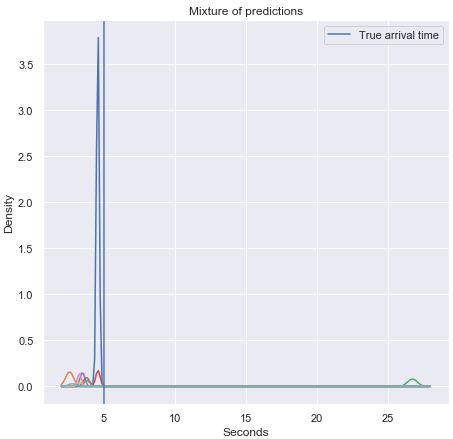
\includegraphics[width=\textwidth]{figures/mixture-end-of-traj.png}
%     \caption{Density of arrival time predictions at 
%       the end of a segment.}\label{fig:mixture-end-of-traj}
%   \end{minipage}
% \end{figure}

\subsection{Event Detection}
The problem of detecting events have not yet been investigated.